%======================================================================
\chapter{Introduction}
\label{ch:intro}
%======================================================================

%----------------------------------------------------------------------
\section{Motivation and Problem Statement}
%----------------------------------------------------------------------
Robotic carts are a prevalent invention designed to aid users in a number of important indoor and outdoor tasks. There are robotic systems currently available in the market that perform these tasks in a variety of ways. For example, in a grocery store, a customer may require the need of more than one cart but cannot push or pull two carts simultaneously. One major drawback, however, is that people with disabilities cannot push one cart let alone have a second cart to carry more items. Moreover, robots used for this purpose are more costly than they are worth.

\vspace*{12pt}
\noindent
In this project, we are proposing a robotic cart that would primarily use analog signals with the use of cost-effective wireless communication to identify the customer and be able to track and follow the customer through the store. The implementation of such a fully functional robotic cart will outreach the scope of the project but is the overall goal for this project in the coming years while encouraging further research in this field.

\vspace*{12pt}
\noindent
Applications of the proposed robotic cart include, but are not limited to, delivery carts to follow mail personnel and carry the deliveries, file transfer carts in offices, hospital carts to aid nurses and doctors by carrying medicine or surgery supplies, and carts in construction sites to carry tools and other supplies across the job site.



%----------------------------------------------------------------------
\section{Literature Review}
%----------------------------------------------------------------------
Abundant research in the field of mobile robotics shows various ways to develop robotic carts that will help consumers in carrying groceries through stores~\cite{Rawashdeh2017-Person,islam_lam_fukuda_kobayashi_kuno_2019,Sales2016-CompaRob}. Currently, the work being done focuses on a few different methods of having a robotic cart interface with the customer and follow them through the store.

\vspace*{12pt}
\noindent
One such method, shown in Fig. \ref{fig:CompaRob}, that has been utilized to make a mobile cart follow a customer through a store is a mobile platform interface that implements ultrasound and radio transmissions technology~\cite{Sales2016-CompaRob}.
\begin{figure}[H]
   \centering
   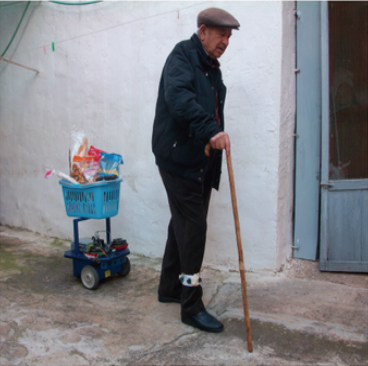
\includegraphics[width=0.4\textwidth]{figs/img/CompaRob}
   \caption{CompaRob Robot}
   \label{fig:CompaRob}
\end{figure}

In the current project, we are implementing XBee S2C RF radios, which are inexpensive and easily configurable, as a remote target device that is carried by the user. The robot will be able to track this remote instead of using line of sight methods~\cite{Miah2018-Intelligent}. In addition to the XBee S2C RF radios, we will equip the robot with a parabolic reflector, which improves radio reception at various distances and angles, \textit{i.e.,} angle of arrivals of RF signals from the remote, based on research done previously in this type of robot localization and mapping~\cite{Miah2018-Intelligent}~\cite{Li2013ANA}.


%----------------------------------------------------------------------
\section{Report Organization}
%----------------------------------------------------------------------
% \begin{itemize}
%     \item Chapter \ref{ch: intro} discusses the background and goals of the project and what other similar projects have accomplished.
%     \item Chapter \ref{ch: sysDesign} explains how the robotic cart system in this project is broken down fundamentally, the components used to build the robot, and the algorithms used to control the robot.
%     \item Chapter \ref{ch: implementation} discusses the implementation of all the parts onto the robot and the experimental results obtained when running the robot.
%     \item Chapter \ref{ch: conclusionAndFuture} concludes the project work and discusses future endeavors on this project.
%     \item Appendix \ref{ch: coppSimModeling} goes through the steps to model and simulate the Budget Bot chassis in CoppeliaSim
%     \item Appendix \ref{ch: assemblyInstructions} gives the step-by-step procedure for assembling the robot
% \end{itemize}

%%% Local Variables:
%%% mode: latex
%%% TeX-master: "../finalReport"
%%% End:
